%% -*- mode: latex; mode: flyspell -*-
\documentclass[12pt, letter]{article}

%% Class name and Assignment number
%%
\newcommand{\courseName}{ECE 435 Medical~Image~Processing}
\newcommand{\assignName}{Assignment~3}

%% Packages
\usepackage{amsmath,amsfonts,amssymb,amsthm,dsfont}
\usepackage{graphicx}
\usepackage[bookmarks=false]{hyperref}
\usepackage{color}
\usepackage{lipsum}
\usepackage{amsmath}

%% Paper format
\usepackage{geometry}
\geometry{
    letterpaper,
    %% total={216mm,279mm}, %< NSERC size
    margin=2.00cm,     %< default
    %% margin=1.87cm,       %< NSERC tightest
}

%% Headers and footers
\usepackage[explicit]{titlesec}
\newpagestyle{titlesec_assignment}{
  \sethead{\courseName}{}{\assignName}\setfoot{}{\thepage}{}
  \headrule
  %% \footrule
}

\begin{document}

%% Set header and footer
\pagestyle{titlesec_assignment}

%% Title
\title{\courseName\\\assignName}
\author{Yiping Wang V00894385}
\maketitle

\paragraph{Question 1: } A non-uniform magnetic field $B$ pointing in the z direction is applied to sample of H+ protons. The field $B$ (in Tesla) varies as a function of $z$ (in cm)

\begin{equation}
    B(z) = 1 + 0.5 \times z
\end{equation}

(a) Find the Larmor frequencies at $z=0$ and and $z=1 cm$.

\paragraph{Answer: } $z=0$
\begin{equation}
    B(0) = 1 + 0.5 \times 0 = 1
\end{equation}
Since the Larmor frequency is given by the following formula:
\begin{equation}
    \omega = \gamma B
\end{equation}

where the gyromagnetic constant $\gamma$ for H+ proton is $42.58 MHz/T$. Therefore, at $z=0$, the Larmor frequency is 

\begin{equation}
    f_0 = 42.58 MHz/T \times 1T = 42.58 MHz
\end{equation}


Similarly, the Larmor frequency at $z=1$ is given as following:

\begin{equation}
    B(1) = 1 + 0.5 \times 1 = 1.5 T
\end{equation}

\begin{equation}
    f_1 = 42.58 MHz/T \times 1.5T = 63.87 MHz
\end{equation}

(b) Suppose at time t=0 two H+ spins located at z=0 and z=1 respectively have the same phase. At what time will these spins be in phase again?

\paragraph{Answer: } The angular frequency is $\omega = 2\pi f$. Since the protons precesses around the $z$ axis with Larmor frequencies, so the
minimum difference in phase for two aligned spins is $2\pi$. Suppose it takes $t
$ to be aligned again, we have the following relationship:

\begin{equation}
    | 2\pi f_0t - 2\pi f_1t | = 2\pi
\end{equation}

Therefore, after some simple algebra, we derive $t=0.0469 \mu s$


\paragraph{Question 2: } Explain the functions of the radio frequency transmit and receive coils in a magnetic resonance imaging system.

\paragraph{Answer: } Radio Frequency (RF) coil can be used as transmitter and receiver. When RF coil is used as transmitter, it generates a second magnetic field ($B_1$), or RF pulse with the same precession frequency, which results in a disturbance of proton alignment with two effects. First, some low energy protons (parallel with the primary magnetic field ($B_0$)) will flip to a high energy state decreasing longitudinal magnetization. Second, protons become synchronized and precess in phase, which will cause the resonance. 

RF coil is also used as receiver to receive signals to create images as protons resume their normal states in the primary magnetic field prior to transmission of the RF pulse, which is a process called relaxation. 

\paragraph{Question 3: } Two fundamental steps during an MRI acquisition process are listed below. Describe and measure the effect each step has on the spins of the hydrogen atoms in the examined object.

(a) Put the object in a spatially constant 3 Tesla magnetic field.

\paragraph{Answer: } By increasing the magnetic field, the magnetization of the ensemble will also increase. Hence, the observed net signal (since more molecules resonating in the magnetic field) from all spins will also increase, which results in accurate anatomic details and reduction in imaging noises.

(b) Send a strong electromagnetic pulse of 127.7 MHz into the object.

\paragraph{Answer: } By sending a strong RF pulse, spins will absorb more energy so that more spins will flip to a higher energy state, which is anti-parallel to the primary magnetic field. In the following relaxation steps, while the spins are returning to the rest states, the spins will release more energy so as to send more signals to the RF receiver. 

\paragraph{Question 4: } The figure below illustrates the process of collecting projections for the generation of a CT image. Considering the same object as in the figure below, draw the diagram that corresponds to the process of image reconstruction via the back-projection algorithm. Explain how the quality of the reconstructed image improves by increasing the number of projections.

\paragraph{Answer: }
Please see Figure~\ref{fig:backproj} for the diagram (next page). 

With more projections, we will obtain a better quality of the reconstructed images. Consider there is only one projection in the horizontal plane, we only get one attenuation coefficient along that projection. Now if we add another projection in the vertical plane, we will get another attenuation coefficient in that direction. Therefore, with more projections, we get a set of attenuation coefficients in respective directions, which then we use back projection algorithms, so we can obtain the specific attenuation coefficient in one specific location. We then can use this information to reconstruct the images to show the contrast between objects. Therefore, with more projections, we get more attenuation coefficients in the object. 


\begin{figure}%
    \centering
    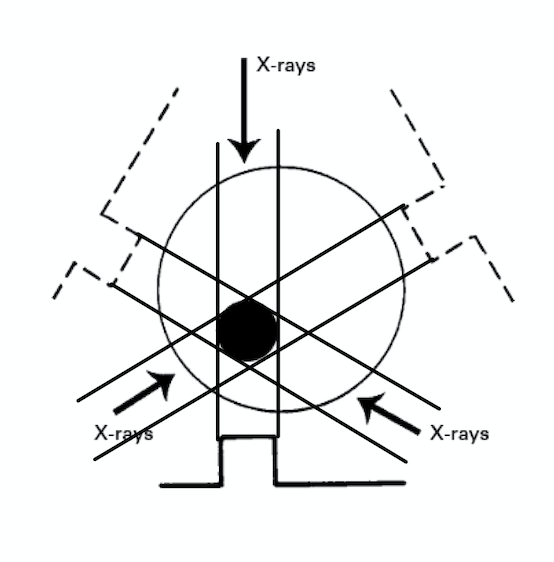
\includegraphics[width=8cm]{backproject_ct.png}
    \caption{Illustration of the process of collecting projections for the generation of a CT image}
    \label{fig:backproj}%
\end{figure}

\paragraph{Question 5: } Explain why the low MHz range is used in ultrasound imaging

\paragraph{Answer: } The depth of penetration of ultrasound depends on the material and is approximately proportional to frequency for most tissues as follows:

\begin{equation}
    d_p \approx \frac{L}{2af}
\end{equation}

where $a$ is an empirical tissue specific coefficient. Therefore, as frequency $f$ increase, the depth of penetration $d_p$ decreases. Although increasing the ultrasound frequency increases spatial resolution, it is more important to reach the required depth to display the anatomical structures of interest.

\paragraph{Question 6:} How much energy is reflected back when an ultrasound pulse passes from muscle to bone? How much is transmitted?

\paragraph{Answer: }
Suppose the transducer launches acoustic waves are normal to the muscle, so the waves that reflect back is about 180 degree to contribute ultrasound imaging. From Table 4.1, the acoustic impedance $Z_1$ for muscle is $1.70 \times 10^6$, and the acoustic impedance $Z_2$ for bone is in the range of $4.8 \times 10^6 \sim 7.8 \times 10^6$. Therefore, the Reflection coefficient can be calculated as follows:

\begin{equation}
R = \frac{(Z_1 - Z_2)^2}{(Z_1 + Z_2)^2}
\end{equation}

\begin{equation}
\begin{split}
\frac{(1.70 \times 10^6 - 4.8 \times 10^6)^2}{(1.70 \times 10^6 + 4.8 \times 10^6)^2} & \leqslant R \leqslant \frac{(1.70 \times 10^6 - 7.8 \times 10^6)^2}{(1.70 \times 10^6 + 7.8 \times 10^6)^2} \\
0.227 & \leqslant R \leqslant 0.412 \\
\end{split}
\end{equation}

Suppose the energy of the incident acoustic waves are $I$. Hence, the energy of the reflect back ultrasound pulse $I_{r}$ is in the following range:

\begin{equation}
0.227I \leqslant I_{r} \leqslant 0.412I\\
\end{equation}

The energy of the transmitted ultrasound pulse $I_t$ is in the following range:

\begin{equation}
0.588I \leqslant I_{t} \leqslant 0.773I\\
\end{equation}

\paragraph{Question 7: } An ultrasound pulse passes through soft tissue and reflects off an interface, producing an echo 0.1 ms later. How deep is the reflecting interface?

\paragraph{Answer: } The velocity of ultrasound pulse is $1540 ms^{-1}$ in soft tissues. We also know that $0.1ms = 10^{-4}s$. Denote the depth of the reflecting surface as $d$.

\begin{equation}
\begin{split}
        d & = \frac{v\times t}{2} \\
          & = \frac{1540 ms^{-1} \times 10^{-4}s}{2} \\
          & = 0.077m
\end{split}
\end{equation}

Hence, the depth of the reflecting surface is $0.077 m$.

\paragraph{Question 8:} If the delay between successive ultrasound pulses is $0.5 ms$, what is the maximum range over which the system can successfully produce images, assuming the speed of the pulses in soft tissue is $1540 ms^{-1}$. Note: The echo from one pulse should be received before the transmission of the next.

\paragraph{Answer: }The pulse repetition interval $T_R$ has a lower bound given by the round trip time to the depth of penetration as follows:

\begin{equation}
    T_R \geqslant \frac{2 \times d_p}{c}
\end{equation}

where $d_p$ denotes the depth of penetration and $c$ denotes the speed of ultrasound pulse. By some simple algebra, we derive:

\begin{equation}
    \begin{split}
            d_p & \leqslant \frac{c \times T_R}{2} \\
                & \leqslant \frac{1540 ms^{-1} \times 0.5 \times 10^{-3}s}{2} \\
                & \leqslant 0.385 m \\
    \end{split}
\end{equation}

Therefore, the maximum range over which the system can successfully produce images is $0.385m$.

\end{document}


%%% Local Variables:
%%% mode: latex
%%% TeX-master: t
%%% End:
